\chapter*{Opis aplikacji}
Po uruchomieniu aplikacji, użytkownikowi najpierw ukazuje się ekran ładowania (przedstawiony na rysunku~\ref{fig:splash}), a następnie menu główne (widoczne na rysunku~\ref{fig:ap1}).
\begin{figure}[h]
	\centering
	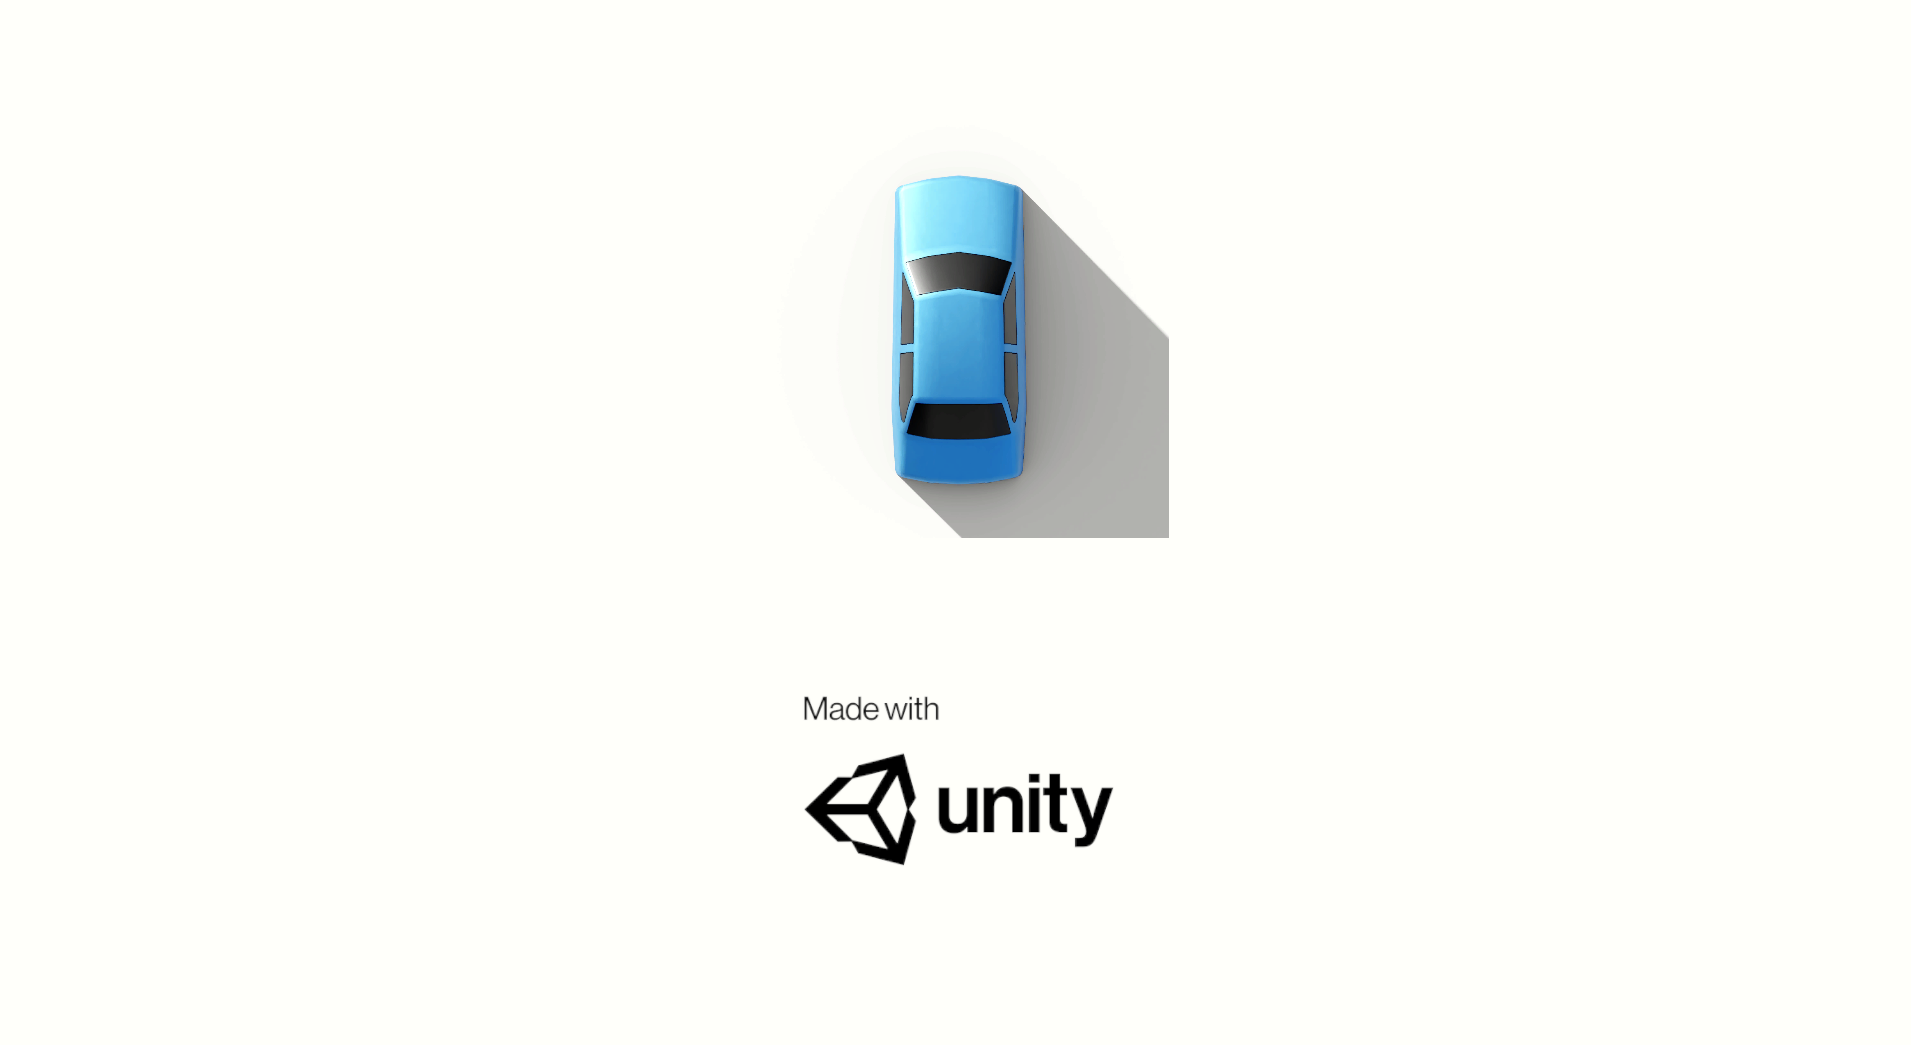
\includegraphics[width=1\linewidth]{splash}
	\caption[Ekran ładowania aplikacji]{Ekran ładowania aplikacji}
	\label{fig:splash}
\end{figure}

\section*{Menu główne}
W górnej części menu znajdują się pola liczbowe, do których użytkownik może wpisać ustawienia symulacji oraz algorytmu ewolucyjnego. Może też skorzystać z ustawień domyślnych. \\Dostępne ustawienia symulacji to:
\begin{itemize}
	\item Prędkość symulacji -- jest to mnożnik prędkości symulowania ruchu drogowego. Przy ustawieniu 1x przeliczane jest 30 kroków symulacji na sekundę. Jedynym górnym ograniczeniem tego ustawienia jest moc obliczeniowa procesora. Domyślna wartość to 100x. \\
	\item Liczba samochodów na pasie -- jest to liczba samochodów, które wjadą na każdy pas ruchu (pasy są widoczne w lewym dolnym rogu rysunku~\ref{fig:ap1}). Domyślna wartość to 20.\\
\end{itemize}
Ustawienia algorytmu ewolucyjnego przedstawiają się następująco:
\begin{itemize}
	\item Populacja pokolenia -- liczba osobników w każdym pokoleniu (stała $n$ w funkcji~\ref{fitness} w poprzednim rozdziale).\\
	\item Liczba pokoleń -- liczba pokoleń, po których proces uczenia ma zostać przerwany. Oprócz tego wpływa na współczynnik mutacji (stała $g$ w funkcji~\ref{mutRate} w poprzednim rozdziale).\\
	\item Długość kroku scenariusza -- zakres, w jakim muszą mieścić się wartości parametrów osobników, a więc długości kroków scenariusza.\\
	\item Maksymalny współczynnik mutacji -- stała $m$ w funkcji~\ref{mutRate} w poprzednim rozdziale.\\
\end{itemize}
\begin{figure}[h]
	\centering
	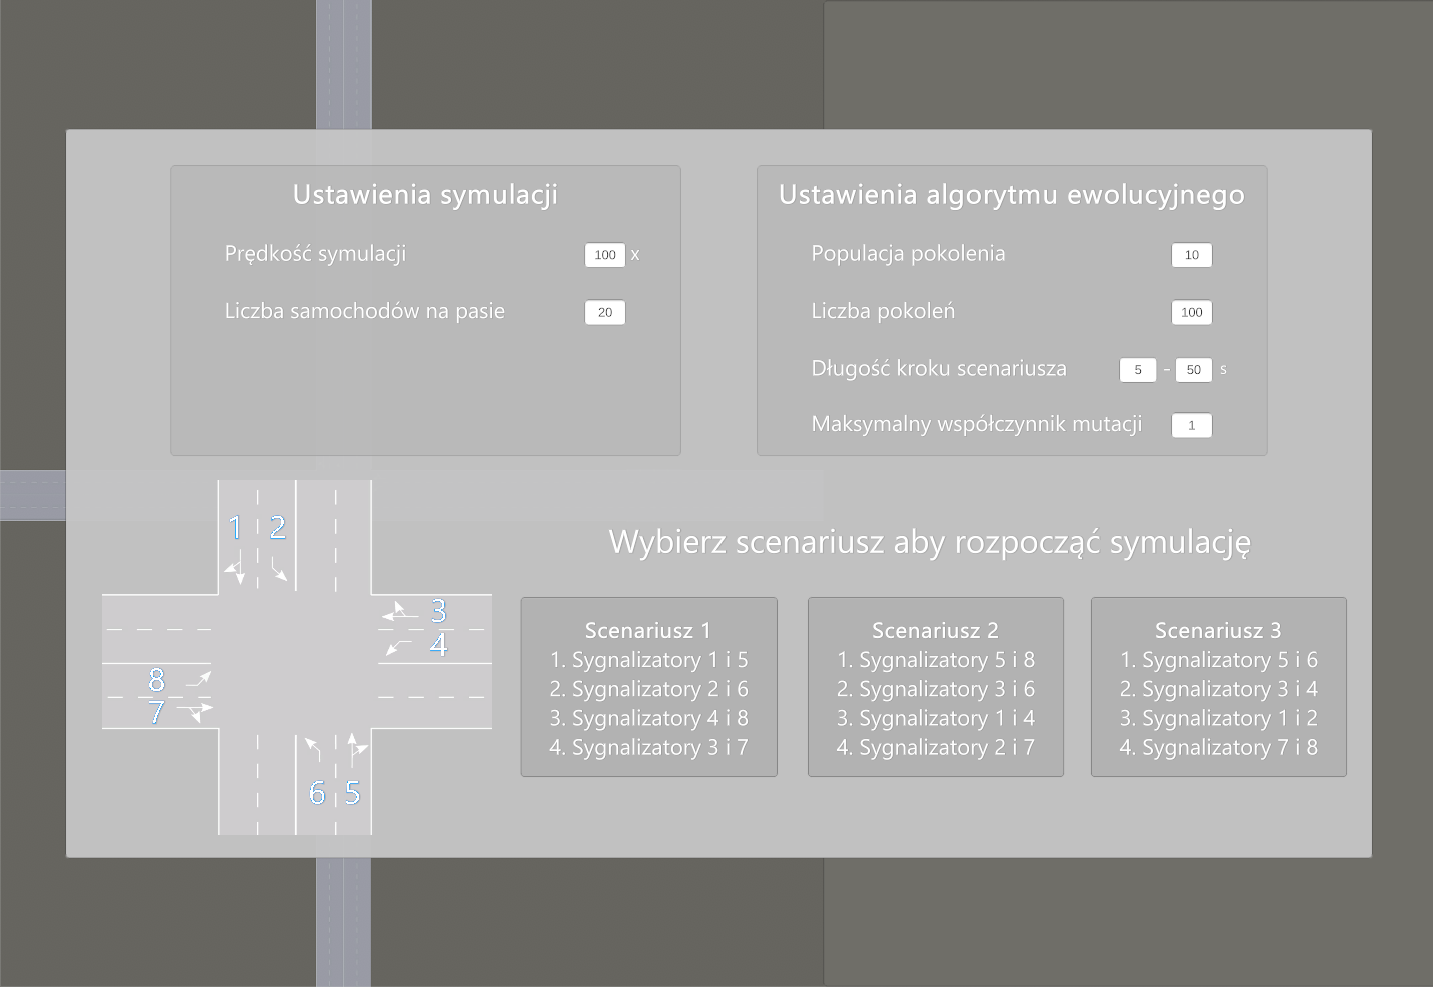
\includegraphics[width=1\linewidth]{ap1}
	\caption[Menu główne aplikacji]{Menu główne aplikacji}
	\label{fig:ap1}
\end{figure}
Po wybraniu ustawień użytkownik musi wybrać scenariusz. Jest to sekwencja sygnalizatorów, które będą zielone w określonym kroku scenariusza. W lewym dolnym rogu menu (na rysunku~\ref{fig:ap1}) widoczny jest schemat z ponumerowanymi sygnalizatorami, mający na celu ułatwienie użytkownikowi zrozumienia różnicy między scenariuszami. 
\section*{Scenariusz} Na przykładzie Scenariusza~1 widocznego w menu: podczas pierwszego kroku scenariusza zielone będą sygnalizatory nr 1 i 5 (oznaczone na schemacie po lewej), pozostałe zaś będą czerwone. Po przejściu do drugiego kroku zielone będą sygnalizatory nr 2 i 6, podczas gdy pozostałe będą czerwone. Analogicznie w kolejnych krokach scenariusza. Długość każdego z tych kroków opisuje obecnie symulowany osobnik.
\section*{Przebieg uczenia i symulacji ruchu}
Po wybraniu scenariusza rozpoczyna się proces uczenia. Aplikację podczas tego procesu przedstawia rysunek~\ref{fig:ap2}. Lewa część ekranu prezentuje postęp symulacji ruchu drogowego z zastosowaniem parametrów obecnie symulowanego osobnika. Z początkiem symulacji osobnika samochody wjeżdżają na skrzyżowanie i poruszają się zgodnie z sygnalizacją. Sygnalizatory przełączają się w odpowiednim czasie, a kiedy skończy się ostatni krok scenariusza, cykl sygnalizacji się zapętla -- wraca do pierwszego kroku. Symulacja trwa tak długo, aż wszystkie samochody opuszczą skrzyżowanie. Wtedy czas trwania symulacji jest zapisywany, zostanie później użyty do oceny dostosowania. Aplikacja przechodzi do symulacji kolejnego osobnika pokolenia -- na skrzyżowanie wjeżdża ta sama liczba samochodów, sygnalizacja zmienia się tym razem w odstępach określonych kolejnym osobnikiem. Cykl powtarza się, aż symulacji poddane zostaną wszystkie osobniki pokolenia. Następnie aplikacja dokonuje oceny i generuje nowe pokolenie, co opisano w rozdziale \textit{Opis teoretyczny algorytmu ewolucyjnego}. Potem odbywa się symulacja osobników nowego pokolenia. Cykl ten powtarza się, aż osiągnięta zostanie liczba pokoleń określona w konfiguracji. \\
Prawa część ekranu przedstawia stan uczenia -- numer obecnego pokolenia i osobnika. Po pierwszym pokoleniu dodatkowo w tej części wyświetlana jest informacja o tym, jaki był czas trwania symulacji najlepszego osobnika poprzedniego pokolenia. Prezentuje to rysunek~\ref{fig:ap3}. Z upływem pokoleń czas symulacji najlepszego osobnika spada, co jest widoczne, jeśli porówna się rysunek~\ref{fig:ap4} do rysunku~\ref{fig:ap3}.
\begin{figure}[h]
	\centering
	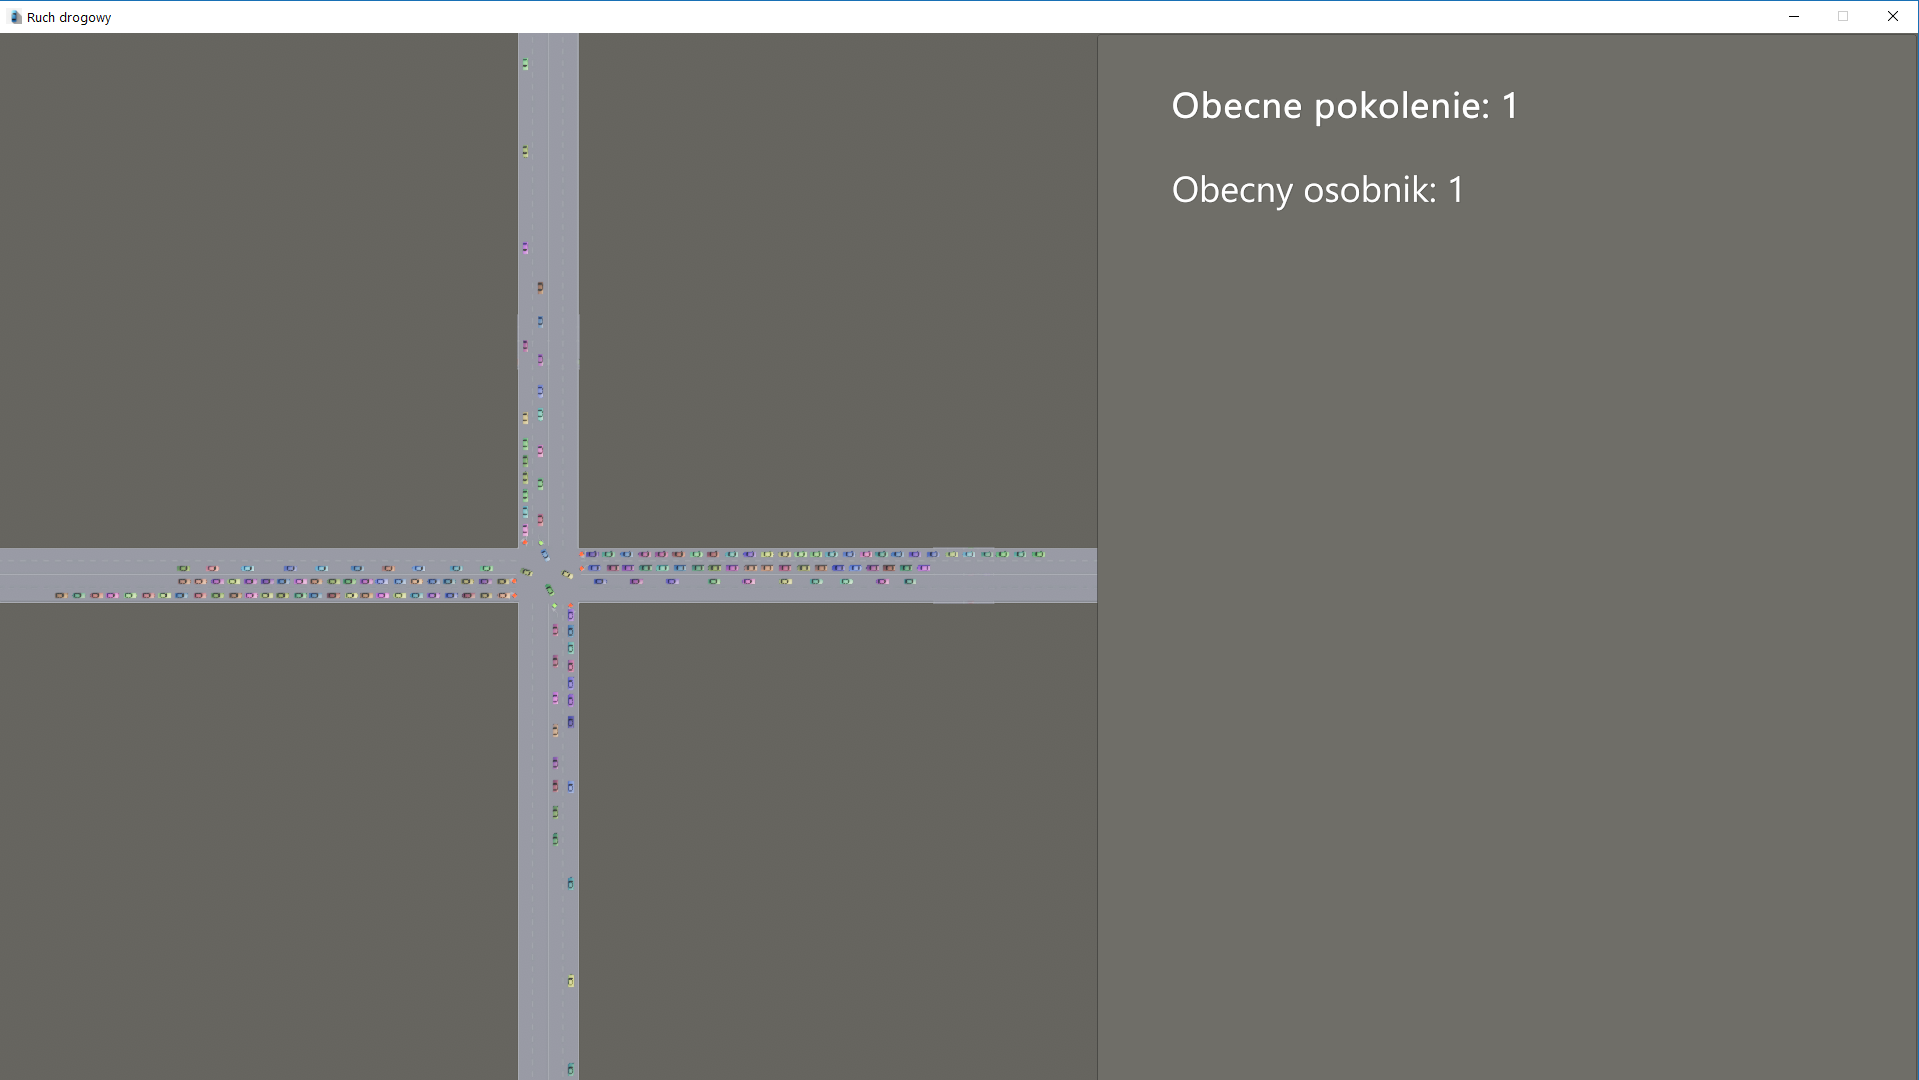
\includegraphics[width=1\linewidth]{ap2}
	\caption[Proces uczenia i symulacji ruchu]{Proces uczenia i symulacji ruchu podczas pierwszego pokolenia}
	\label{fig:ap2}
\end{figure}
\begin{figure}
	\centering
	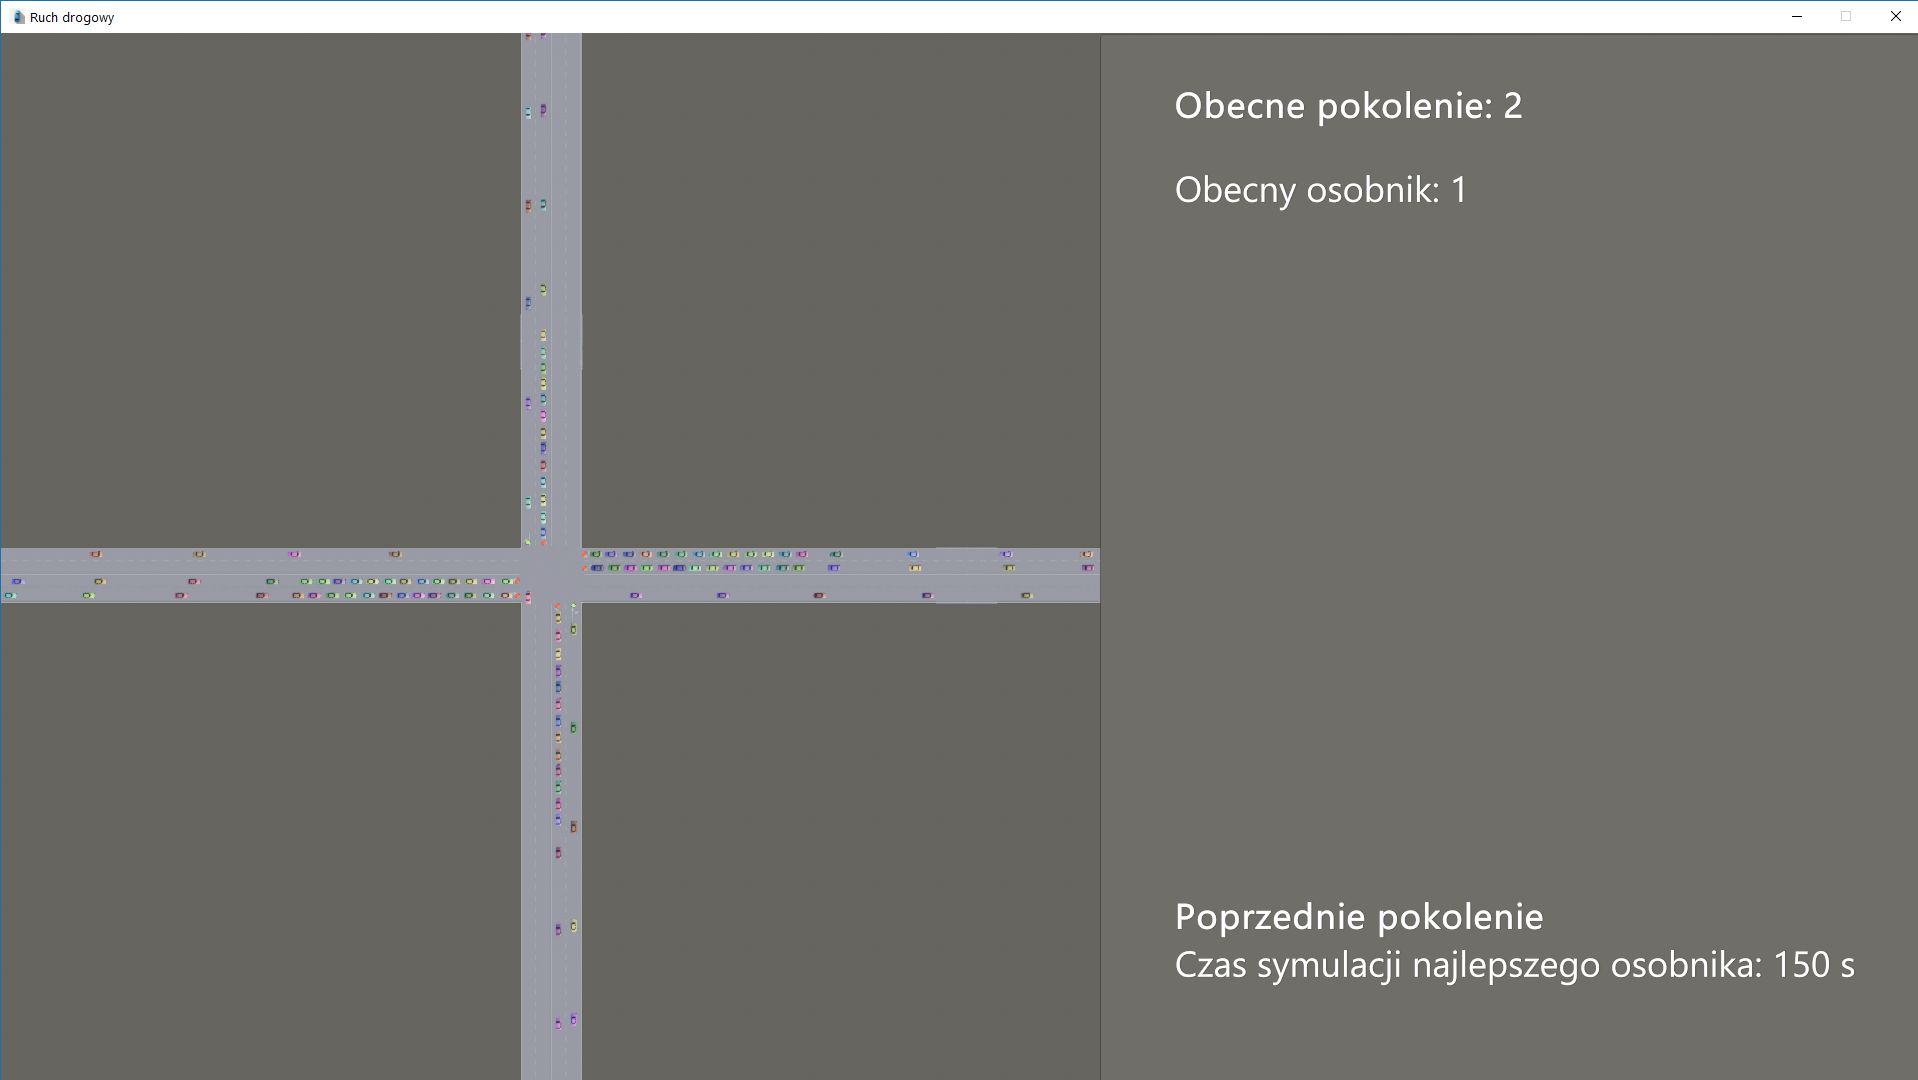
\includegraphics[width=1\linewidth]{ap3}
	\caption[Proces uczenia i symulacji ruchu]{Proces uczenia i symulacji ruchu podczas drugiego pokolenia}
	\label{fig:ap3}
\end{figure}
\begin{figure}
	\centering
	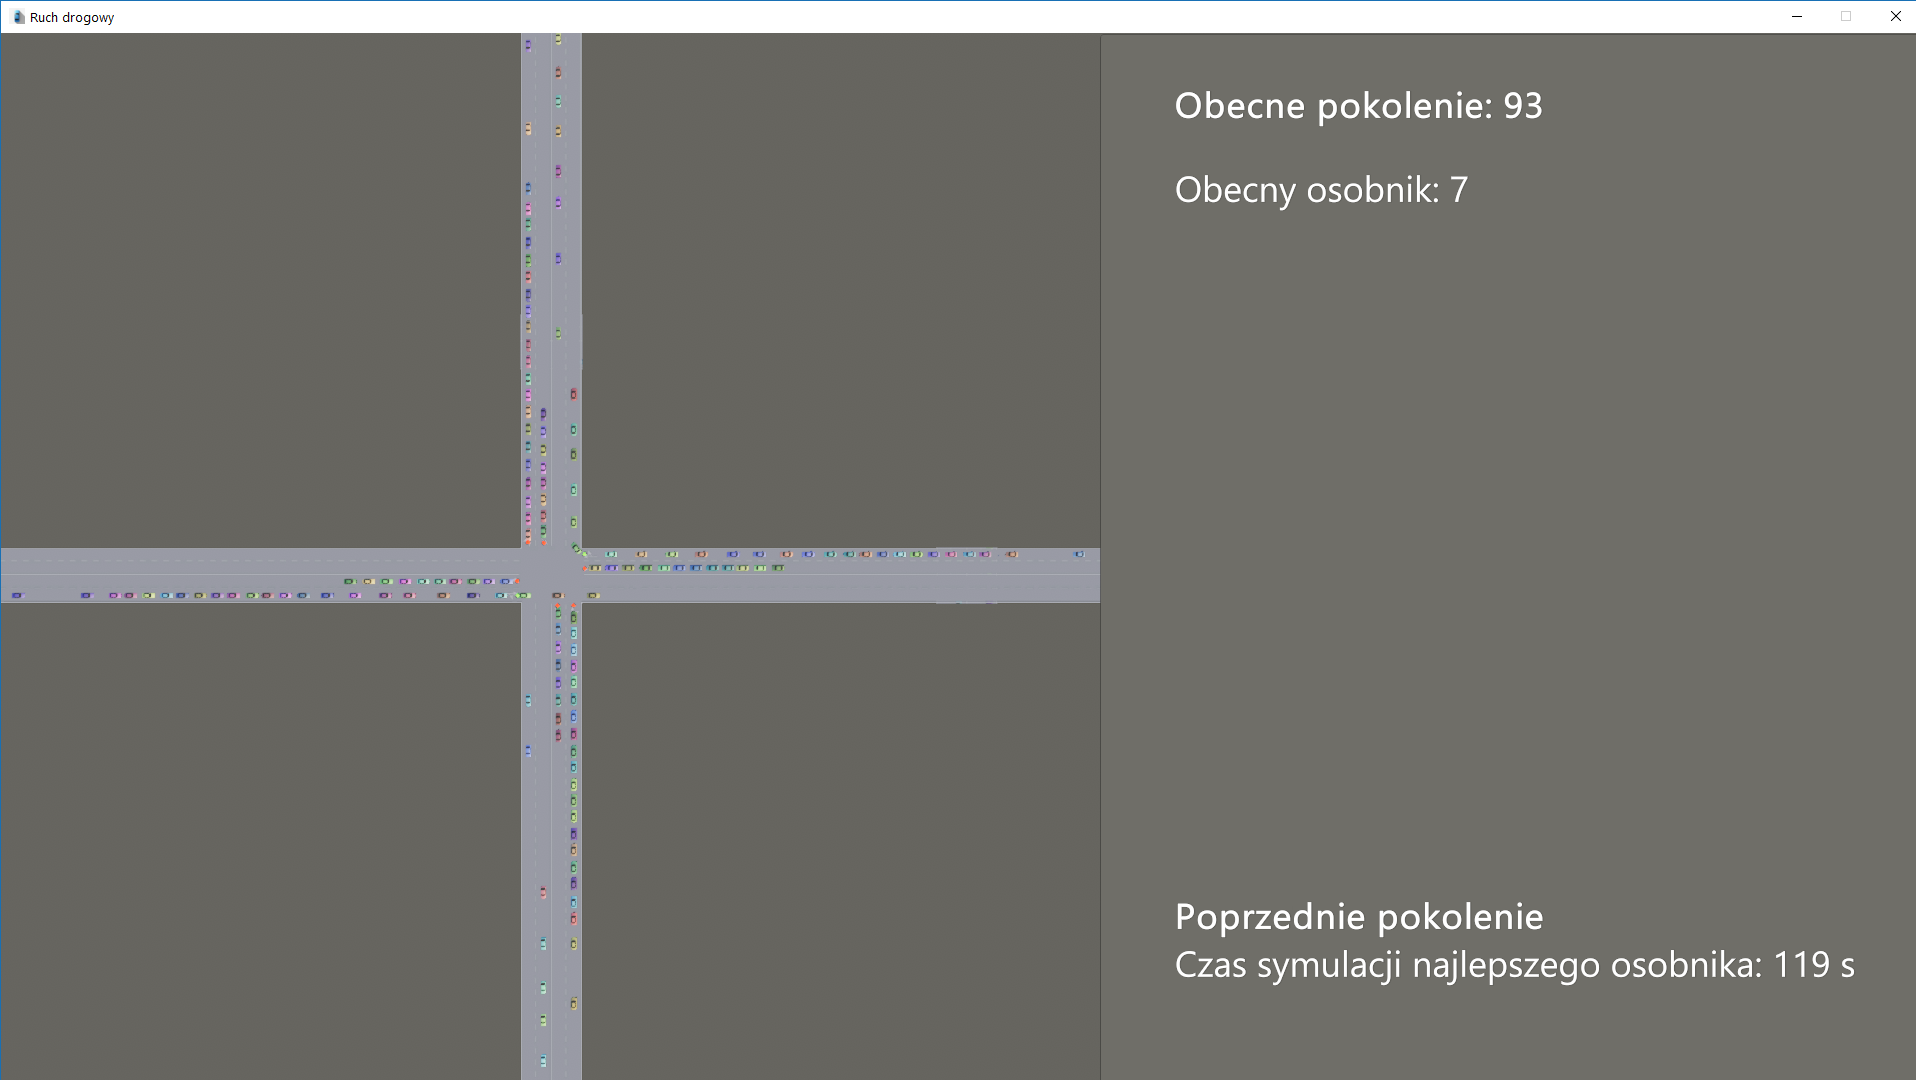
\includegraphics[width=1\linewidth]{ap4}
	\caption[Proces uczenia i symulacji ruchu]{Proces uczenia i symulacji ruchu podczas 93. pokolenia}
	\label{fig:ap4}
\end{figure}
\section*{Ekran końcowy}
Po ukończeniu procesu uczenia użytkownikowi ukazuje się ekran końcowy (widoczny na rysunku~\ref{fig:ap9}), który przedstawia wyniki uczenia. Informacje prezentowane na tym ekranie to czas trwania symulacji najlepszego osobnika ostatniego pokolenia i jego parametry. Na tym ekranie znajduje się również przycisk \textit{Wyjdź}, który pozwala na zamknięcie aplikacji.
\begin{figure}
	\centering
	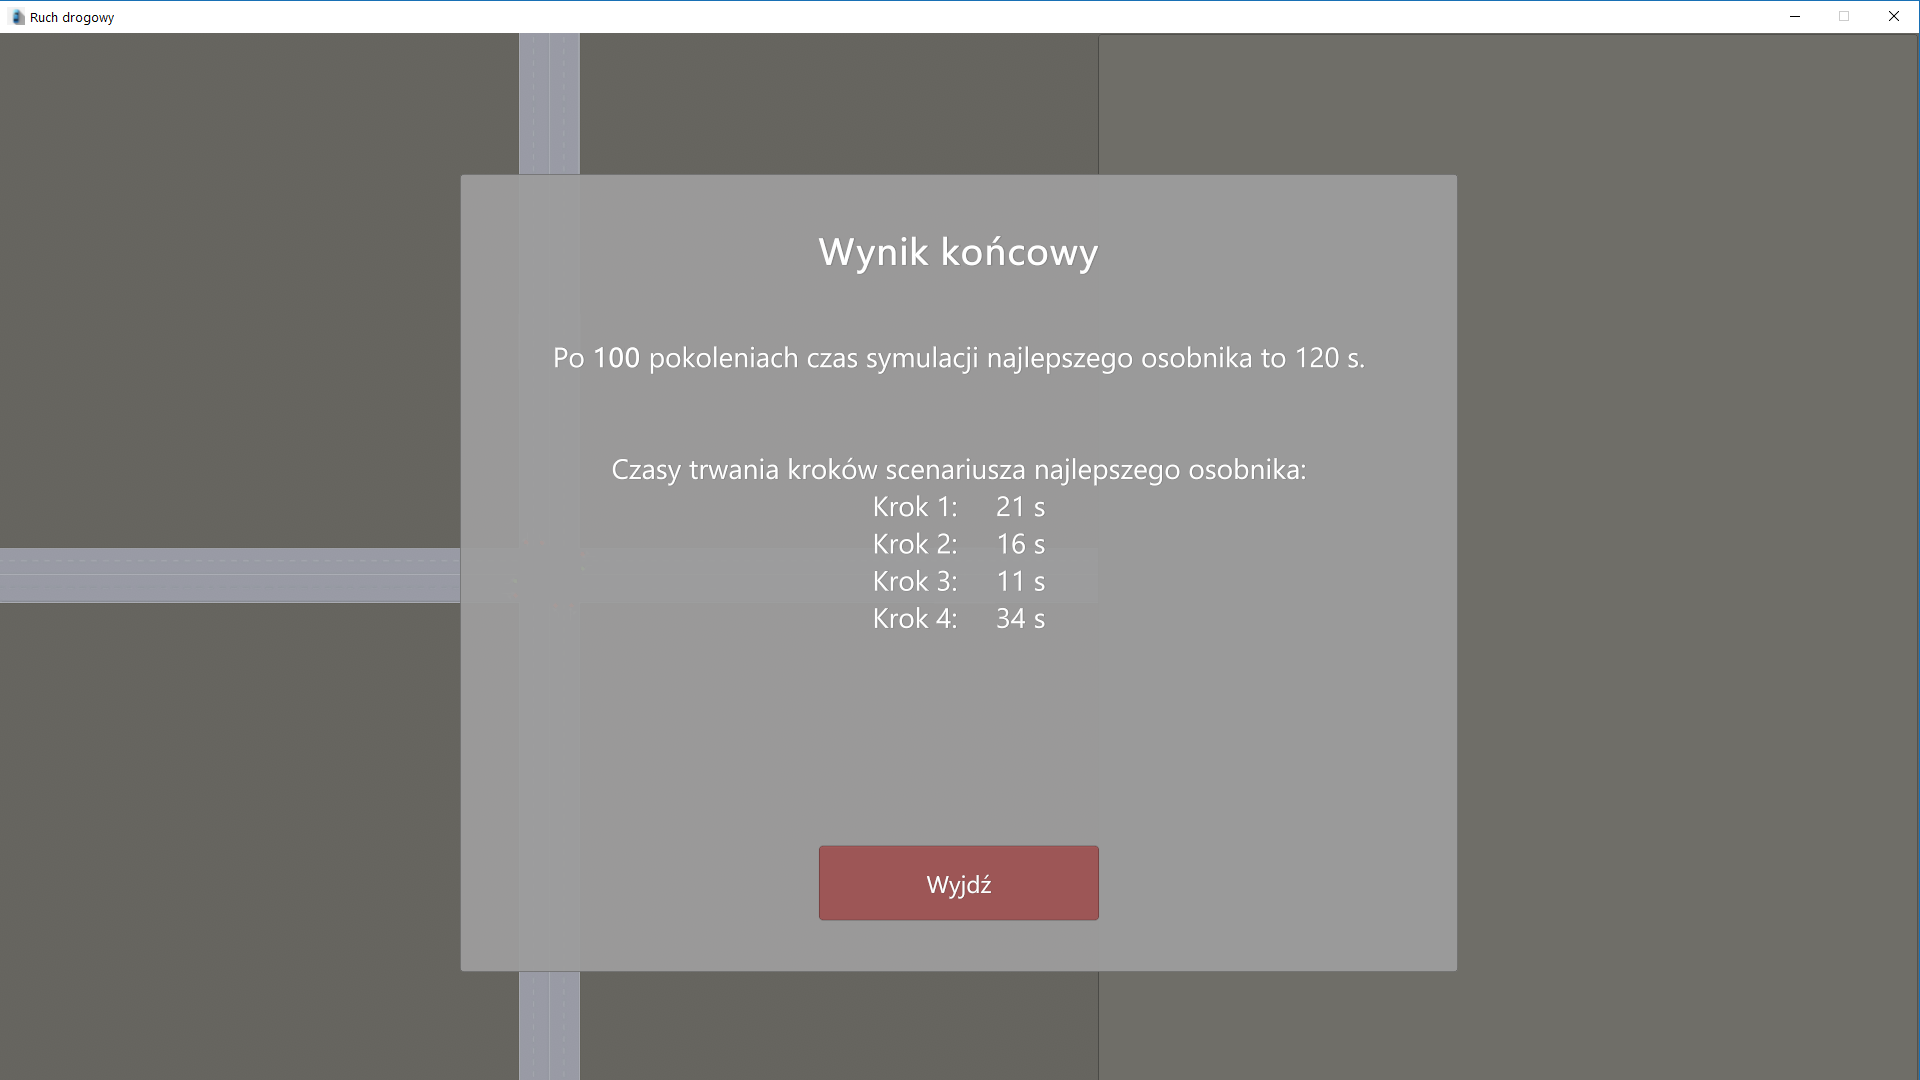
\includegraphics[width=1\linewidth]{ap9}
	\caption[Ekran końcowy]{Ekran końcowy}
	\label{fig:ap9}
\end{figure}

\section*{Ruch pojazdów}
Każdy pojazd porusza się wzdłuż jednej z 12 krzywych sklejanych -- przykładową przedstawiono na rysunku~\ref{fig:ap7} kolorem zielonym. Każda z nich składa się z krzywych Béziera drugiego stopnia.
\section*{Dodatkowe proste narzędzia}Przy okazji powstawania tej aplikacji stworzono proste narzędzie do modyfikacji krzywych sklejanych. Pozwala ono w łatwy sposób przesuwać ich punkty kontrolne w trybie graficznym (co przedstawiono na rysunku~\ref{fig:ap6}) lub wprowadzając ich współrzędne (co ukazuje rysunek~\ref{fig:ap7}).
\paragraph{}Stworzono również narzędzie do szybkiego tworzenia scenariuszy, widoczne na rysunku~\ref{fig:ap8}. Pozwala ono określić liczbę kroków i listę sygnalizatorów, które będą w danym kroku zielone.
\paragraph{}Narzędzia te skróciły czas potrzebny na przygotowanie aplikacji i ułatwiły testowanie różnych rozwiązań.
\begin{figure}
	\centering
	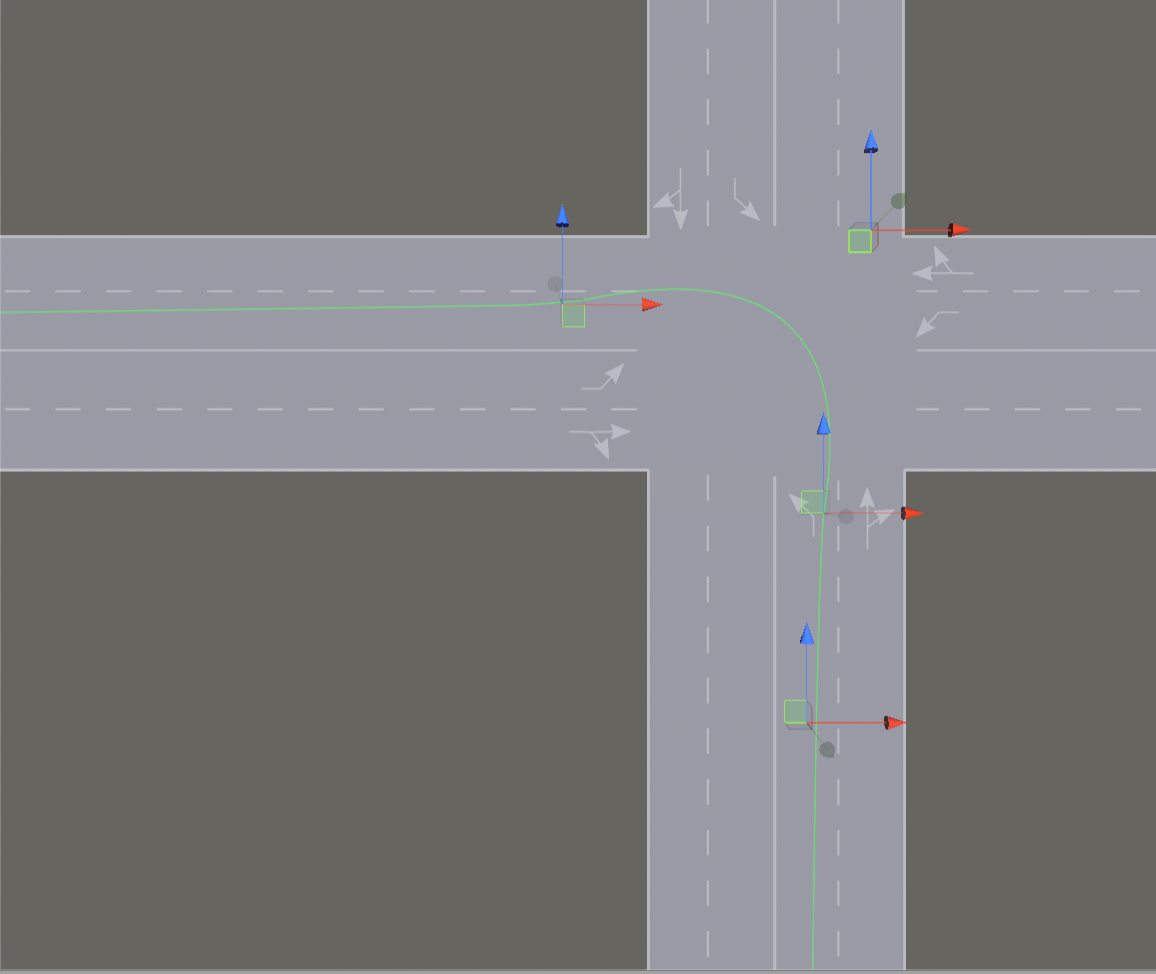
\includegraphics[width=1\linewidth]{ap6}
	\caption[Narzędzie do modyfikacji krzywych sklejanych w trybie graficznym]{Narzędzie do modyfikacji krzywych sklejanych w trybie graficznym}
	\label{fig:ap6}
\end{figure}
\begin{figure}
	\centering
	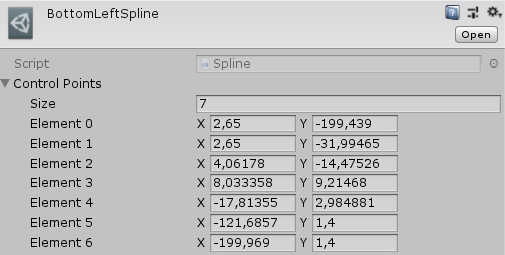
\includegraphics[width=0.8\linewidth]{ap7}
	\caption[Narzędzie do modyfikacji krzywych sklejanych w trybie tekstowym]{Narzędzie do modyfikacji krzywych sklejanych w trybie tekstowym}
	\label{fig:ap7}
\end{figure}
\begin{figure}
	\centering
	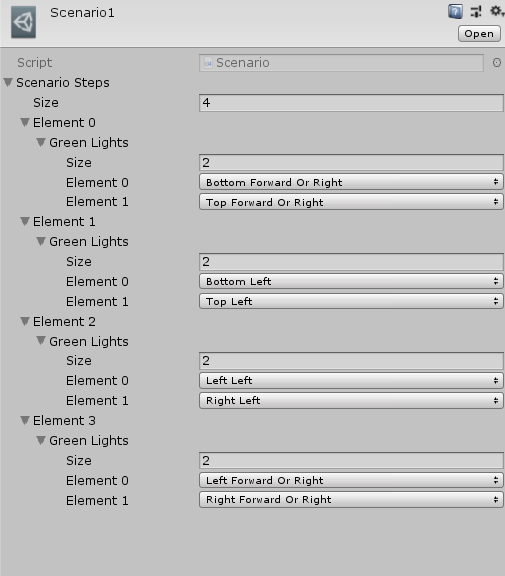
\includegraphics[width=0.8\linewidth]{ap8}
	\caption[Narzędzie do tworzenia scenariuszy]{Narzędzie do tworzenia scenariuszy}
	\label{fig:ap8}
\end{figure}
%Kolejny rozdział wyniki: głównie wykresy
%Podsumowanie
%Streszczenie, abstract i dopisać do wstępu opis rozdziałów



